%%%%%%%%%%%%%%%%%%%%%%%%%%%%%%%%%%%%%%%%%
% Simple Sectioned Essay Template
% LaTeX Template
%
% This template has been downloaded from:
% http://www.latextemplates.com
%
% Note:
% The \lipsum[#] commands throughout this template generate dummy text
% to fill the template out. These commands should all be removed when 
% writing essay content.
%
%%%%%%%%%%%%%%%%%%%%%%%%%%%%%%%%%%%%%%%%%

%----------------------------------------------------------------------------------------
%	PACKAGES AND OTHER DOCUMENT CONFIGURATIONS
%----------------------------------------------------------------------------------------

\documentclass[12pt]{article} % Default font size is 12pt, it can be changed here

\usepackage{geometry} % Required to change the page size to A4
\geometry{a4paper} % Set the page size to be A4 as opposed to the default US Letter

\usepackage{graphicx} % Required for including pictures
\usepackage[utf8]{inputenc}
\usepackage[T1]{fontenc}
\usepackage{float} % Allows putting an [H] in \begin{figure} to specify the exact location of the figure
\usepackage{wrapfig} % Allows in-line images such as the example fish picture
\usepackage[portuguese]{babel}
\usepackage{natbib}
\usepackage{multirow}
\usepackage{changepage}




\usepackage{lipsum} % Used for inserting dummy 'Lorem ipsum' text into the template

\usepackage{makecell}

\renewcommand\theadalign{cb}
\renewcommand\theadfont{\bfseries}
\renewcommand\theadgape{\Gape[4pt]}
\renewcommand\cellgape{\Gape[4pt]}

\linespread{1.2} % Line spacing

%\setlength\parindent{0pt} % Uncomment to remove all indentation from paragraphs

\graphicspath{{Pictures/}} % Specifies the directory where pictures are stored
\addto\captionsportuguese{\renewcommand*\contentsname{Indíce} }


\begin{document}

%----------------------------------------------------------------------------------------
%	TITLE PAGE
%----------------------------------------------------------------------------------------

\begin{titlepage}

\newcommand{\HRule}{\rule{\linewidth}{0.5mm}} % Defines a new command for the horizontal lines, change thickness here

\center % Center everything on the page

\textsc{\LARGE Universidade Estadual de Campinas}\\[1.5cm] % Name of your university/college
\textsc{\Large Faculdade de Engenharia Mecânica}\\[0.5cm] % Major heading such as course name

\HRule \\[0.4cm]
{ \huge \bfseries TG: Relatório Parcial}\\[0.4cm] % Title of your document
\HRule \\[1cm]

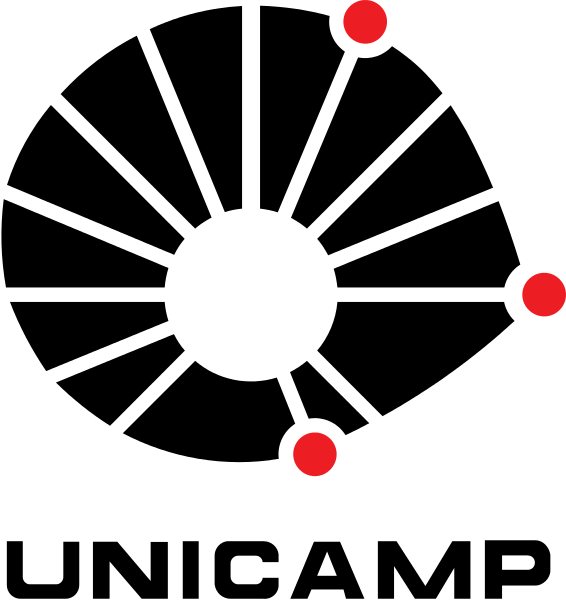
\includegraphics[scale=0.3]{pictures/unicamp.png}\\
\vspace{12mm}


\begin{minipage}{0.4\textwidth}
\begin{flushleft} \large
\emph{Autor:}\\
Henrique de Abreu {Amitay} % Your name
\end{flushleft}
\end{minipage}
~
\begin{minipage}{0.4\textwidth}
\begin{flushleft} \large
\emph{Orientador:} \\
André Ricardo Fioravanti % Supervisor's Name
\end{flushleft}
\end{minipage}\\[4cm]

{\today}\\[3cm] % Date, change the \today to a set date if you want to be precise

%\includegraphics{Logo}\\[1cm] % Include a department/university logo - this will require the graphicx package

\vfill % Fill the rest of the page with whitespace

\end{titlepage}

\tableofcontents
\pagebreak

%----------------------------------------------------------------------------------------
%	OBJETIVO
%----------------------------------------------------------------------------------------

\section{Objetivo}

\paragraph{}O trabalho aqui descrito tem como objetivo propor uma reformulação do curso de Engenharia de Controle e Automação da Universidade Estadual de Campinas, de forma a se ter um curso mais alinhado com as competências esperadas de um engenheiro pleno. Este trabalho foi motivado pela observação do autor de que um número considerável de alunos, ao se aproximar do fim de seus cursos, não demonstravam conhecimento prático básico esperados de um engenheiro, além de terem tido pouquíssimas experiências com desenvolvimento e gerenciamento de projetos. Existe também um Grupo de Trabalho (GT) na Faculdade de Engenharia Mecânica responsável por discutir e formular mudanças no curriculo atual dos cursos oferecidos pela faculdade. Espera-se que este trabalho seja agregador ao que é desenvolvido nesse GT.

\paragraph{}Planeja-se que esta reformulação, inicialmente se dê pela criação de disciplinas de projeto, onde os alunos deverão desenvolver projetos práticos a partir de conhecimento adquirido no curso, periodicamente.

%----------------------------------------------------------------------------------------
%	MÉTODO E CRONOGRAMA
%----------------------------------------------------------------------------------------

\section{Método}

Inicialmente, antes de qualquer proposta, espera-se fazer estudos preliminares de forma a se definir exatamente o que será proposto, logo em um momento inicial planeja-se:

\begin{itemize}
\setlength\itemsep{0.01mm}
\item Definir exatamente o escopo e as competências esperadas de um engenheiro recém formado.
\item Analisar a grade do curso de Engenharia de Controle e Automação da Unicamp e apontar as competências desenvolvidas em cada uma das disciplinas.
\item Estudar outras instituições de ensino, tanto no Brasil quanto no exterior, que desenvolveram projetos parecidos de ensino.
\end{itemize}

\paragraph{} Tendo definido estes pontos, a segunda etapa do trabalho consistirá em propor diferentes projetos, ou modelos de projetos que explorem todas as competências apontadas. Além disso será necessário analisar a viabilidade destes projetos, tendo como base a infraestrutura da universidade e o impacto que isto pode causar no currículo academico. Em suma, planeja-se:

\begin{itemize}
\setlength\itemsep{0.01mm}
\item Agrupar as competências apontadas nos estudos preliminares em grupos, baseados em qual período o aluno estará.
\item Propor projetos ou modelos de projetos que englobem estas competencias.
\item Analisar a viabilidade destes projetos e caso não seja viável, propor alguma alternativa.
\end{itemize}

\section{Cronograma}

Espera-se que este trabalho seja feito durante o peŕiodo de um ano, entre julho de 2017 até junho de 2018. A primeira etapa do trabalho será feita durante o segundo semestre de 2017 e a segunda etapa será feita no primeiro semestre de 2018. Estipulou-se o seguinte cronograma:

\begin{table}[H]
\centering
\begin{tabular}{|l|p{0.8\linewidth}|}
\hline
\multicolumn{1}{|c|}{\textbf{Período}} & \multicolumn{1}{c|}{\textbf{Etapa}}                                                   \tabularnewline \hline
Julho/2017                                              & Finalização do planejamento do trabalho
\tabularnewline \hline
Agosto/2017                                           & Definição do escopo e competências de um engenheiro
\tabularnewline \hline
Setembro/2017                                       & Analisar a grade do curso de Engenharia de Controle e Automação e apontar competências
\tabularnewline \hline
Outubro/2017                      		& Estudar outras instuições de ensino
\tabularnewline \hline
Novembro/2017                      		& Compilação e escrita das informações apontadas nas etapas passadas e revisão bibliográfica                                                                                                     \tabularnewline \hline	
Dezembro/2017                                       & Revisão do trabalho desenvolvido até então
\tabularnewline \hline
Janeiro/2018                                           & Agrupar as competências apontadas em grupos
\tabularnewline \hline
Fevereiro/2018                                       & Propor projetos ou modelos de projetos
\tabularnewline \hline
Março/2018                                             & Compilação e escrita dos projetos propostos
\tabularnewline \hline
Abril/2018                                            	& Analisar a viabilidade destes projetos e caso não sejá viavel propor alguma alternativa.
\tabularnewline \hline
Maio/2018                                            	& Revisão do trabalho desenvolvido até então
\tabularnewline \hline
Junho/2018                                            	& Finalização da escrita do trabalho.

\tabularnewline \hline
\end{tabular}
\end{table}

%----------------------------------------------------------------------------------------
%	DEFINIÇÃO DO ESCOPO
%----------------------------------------------------------------------------------------
\section{Escopo do Engenheiro de Controle e Automação}
\subsection{Definição de Engenharia de Controle e Automação}

 \paragraph{}Engenharia de Controle e Automação, ou Mecatrônica, é um campo relativamente jovem da engenharia. O avanço nas áreas de computação, semicondutores, sistemas embarcados e controle no último século criaram solo fértil para um campo novo e cheio de possibilidades. Porém, como é uma área nova ainda  não existe consenso no escopo esperado de um engenheiro de Controle e Automação.

\paragraph{}A definição de Mecatrônica vem sendo alterada com os anos. Sua definição original foi feita pela \textit{Yasakawa Electric Company}, que a definiu como: 

\paragraph{}\textit{"A palavra, mecatrônica, é composta de "meca" de mecanismo e "trônica" de eletrônica. Em outras palavras, tecnologias e produtos desenvolvidos irão incorporar sistemas eletrônicos em mecanismos cada vez mais, de maneira orgânica e intima, fazendo com que seja impossível dizer onde um começa e outro termina."}

\paragraph{}Está definição vem evoluindo conforme mais estudos são desenvolvidos na área. Uma das definições mais atuais foi definida por W.Bolton: 

\paragraph{}\textit{"Um sistema mecatrônico não é apenas o casamento de sistemas elétricos e mecânicos e é mais que apenas um sistema de controle; é a integração completa de todos eles."}

\paragraph{}As muitas definições existentes mostram o quanto o campo de Controle e Automação é novo e o quanto ele tem evoluído com os avanços tecnológicos, porém o que fica mais evidenciado é que independente da definição o campo exige que o engenheiro tenha um rol vasto e variado de competências.

\paragraph{}É necessário então que estas competências sejam levantadas e analisadas de forma a entender melhor como o curso oferecido pela UNICAMP desenvolve tais habilidades.


\subsection{Levantamento das competências de um Engenheiro}
\paragraph{}Para este estudo, a Engenharia de Controle e Automação pode ser dividida nos seguintes pontos chave:

\begin{itemize}
\setlength\itemsep{0.01mm}
\item Modelagem de sistemas físicos
	\subitem Para este estudo, este item será dividido em Sistemas Mecânicos e Sistemas Elétricos.
\item Sensores e Atuadores
\item Sinais e Sistemas
\item Computadores e Sistemas Lógicos
\item Software e Aquisição de Dados
\end{itemize}

\paragraph{}Os itens acima descrevem os campos que, teoricamente, definem o campo de Engenharia de Controle e Automação, porém, é preciso também apontar as competências esperadas de um engenheiro, seja ele de Controle e Automação ou não.

\paragraph{}O estudo feito por Male em 2012, aponta as seguintes competências esperadas de um engenheiro:

\begin{itemize}
\setlength\itemsep{0.01mm}
\item Comunicação
\item Trabalho em Equipe
\item  Profissionalismo
\item Autonomia
\item Ingenuidade
\item Liderança e Gestão
\item Engenharia voltada à negócios
\item Empreendedorismo
\item Engenharia prática
\item Responsabilidades profissionais
\item Aplicação de teoria técnica
\end{itemize}

\paragraph{}Por questões de simplicidade estas competências serão agrupadas e referidas como: \textit{Competências não técnicas}, já que se referem à competências voltadas mais à postura do que conhecimentos acadêmicos.

\paragraph{}OBS: Alguns desses pontos podem parecer mais alinhados com o mercado e indústria e divergente da realidade acadêmica. É importante frisar que este estudo busca um perfil de engenheiro pleno, que possa atuar tanto em ambientes acadêmicos quanto ambientes da indústria.

\paragraph{}Por fim, as competências que serão usadas como base neste estudo são:

\begin{itemize}
\setlength\itemsep{0.01mm}
\item Modelagem de Sistemas Mecânicos
\item Modelagem de Sistemas Elétricos
\item Sensores e Atuadores
\item Sinais e Sistemas
\item Computação e Sistemas Lógicos
\item Software e Aquisição de Dados
\item Competências não técnicas
\end{itemize}

%----------------------------------------------------------------------------------------
%	Análise do curriculo
%----------------------------------------------------------------------------------------

\section{Análise do currículo atual}

\paragraph{}O catálogo atual do curso de Engenharia de Controle e Automação apresenta, na sua versão mais recente, 246 hora-aula/semana (créditos), divididos em uma grade de 12 semestres.  As disciplinas oferecidas podem ser cursadas em qualquer ordem, dado que respeitem uma sequência de pré-requisitos estabelecidos, porém para esta análise irá ser considerada a integralização sugerida pela faculdade. Dentro destes 246 créditos, 12 são de disciplinas eletivas.

\paragraph{} O currículo pleno, com seus respectivos semestres indicados:

% Please add the following required packages to your document preamble:
% \usepackage{multirow}
\begin{table}[H]
\centering
\begin{tabular}{|c|l|c|}
\hline
Semestre             & Disciplina                                                 & Créditos \\ \hline
\multirow{5}{*}{1o}  & Cálculo I                                                  & 6        \\ \cline{2-3} 
                     & Química                                                    & 4        \\ \cline{2-3} 
                     & Introdução à Engenharia de Controle e Automação            & 2        \\ \cline{2-3} 
                     & Geometria Analítica e Vetores                              & 4        \\ \cline{2-3} 
                     & Física Geral I                                             & 4        \\ \hline
\multirow{5}{*}{2o}  & Cálculo II                                                 & 6        \\ \cline{2-3} 
                     & Física Geral III                                           & 4        \\ \cline{2-3} 
                     & Desenho Técnico Assistido por Computador                   & 4        \\ \cline{2-3} 
                     & Oficinas - Mecatrônica                                     & 4        \\ \cline{2-3} 
                     & Algoritmos e Programação de Computadores                   & 6        \\ \hline
\multirow{5}{*}{3o}  & Cálculo III                                                & 6        \\ \cline{2-3} 
                     & Estruturas de Dados                                        & 6        \\ \cline{2-3} 
                     & Física Experimental I                                      & 2        \\ \cline{2-3} 
                     & Circuitos Elétricos                                        & 4        \\ \cline{2-3} 
                     & Materiais de Engenharia                                    & 2        \\ \hline
\multirow{5}{*}{4o}  & Cálculo Numérico                                           & 4        \\ \cline{2-3} 
                     & Álgebra Linear                                             & 4        \\ \cline{2-3} 
                     & Programação Orientada a Objetos                            & 4        \\ \cline{2-3} 
                     & Termodinâmica I                                            & 4        \\ \cline{2-3} 
                     & Estática                                                   & 4        \\ \hline
\multirow{5}{*}{5o}  & Mecânica dos Fluidos I                                     & 4        \\ \cline{2-3} 
                     & Organização Básica de Computadores e Linguagem de Montagem & 4        \\ \cline{2-3} 
                     & Dinâmica                                                   & 4        \\ \cline{2-3} 
                     & Eletrônica Aplicada                                        & 4        \\ \cline{2-3} 
                     & Estatística para Experimentalistas                         & 4        \\ \hline
\multirow{6}{*}{6o}  & Laboratório de Eletrônica Aplicada                         & 2        \\ \cline{2-3} 
                     & Circuitos II                                               & 4        \\ \cline{2-3} 
                     & Análise Linear de Sistemas                                 & 4        \\ \cline{2-3} 
                     & Engenharia de Fabricação                                   & 2        \\ \cline{2-3} 
                     & Transferência de Calor I                                   & 4        \\ \cline{2-3} 
                     & Circuitos Lógicos                                          & 4        \\ \hline
\multirow{6}{*}{7o}  & Fabricação Mecânica e Metalúrgica                          & 2        \\ \cline{2-3} 
                     & Laboratório de Circuitos Lógicos                           & 2        \\ \cline{2-3} 
                     & Sistemas Fluidotérmicos I                                  & 4        \\ \cline{2-3} 
                     & Resistência dos Materiais I                                & 4        \\ \cline{2-3} 
                     & Projeto de Sistemas Computacionais                         & 4        \\ \cline{2-3} 
                     & Vibrações de Sistemas Mecânicos                            & 4        \\ \hline
\end{tabular}
\caption{Catálogo atual do curso -  Parte 1}
\label{catalago1}
\end{table}

\begin{table}[H]
\centering
\begin{tabular}{|c|l|c|}
\hline
Semestre             & Disciplina                                                 & Créditos \\ \hline
\multirow{6}{*}{8o}  & Controle de Sistemas Mecânicos                             & 4        \\ \cline{2-3} 
                     & Resistência dos Materiais II                               & 4        \\ \cline{2-3} 
                     & Princípios de Conversão de Energia                         & 4        \\ \cline{2-3} 
                     & Instrumentação Básica                                      & 2        \\ \cline{2-3} 
                     & Laboratório de Ensaio dos Materiais                        & 2        \\ \cline{2-3} 
                     & Sistemas de Aquisição de Dados                             & 4        \\ \hline
\multirow{6}{*}{9o}  & Projeto de Sistemas Embarcados                             & 4        \\ \cline{2-3} 
                     & Eletrônica para Automação Industrial                       & 4        \\ \cline{2-3} 
                     & Laboratório de Dispositivos Eletromecânicos                & 2        \\ \cline{2-3} 
                     & Planejamento e Controle da Produção I                      & 4        \\ \cline{2-3} 
                     & Modelagem de Dispositivos Eletromecânicos                  & 2        \\ \cline{2-3} 
                     & Robótica Industrial                                        & 4        \\ \hline
\multirow{5}{*}{10o} & Sistemas Mecânicos                                         & 4        \\ \cline{2-3} 
                     & Laboratório de Eletrônica para Automação Industrial        & 2        \\ \cline{2-3} 
                     & Automação Industrial                                       & 4        \\ \cline{2-3} 
                     & Controle Avançado de Sistemas                              & 4        \\ \cline{2-3} 
                     & Laboratório de Sistemas Embarcados                         & 2        \\ \hline
\multirow{4}{*}{11o} & Ciências do Ambiente                                       & 2        \\ \cline{2-3} 
                     & Laboratório de Controle de Sistemas                        & 2        \\ \cline{2-3} 
                     & Laboratório de Automação Industrial                        & 2        \\ \cline{2-3} 
                     & Trabalho de Graduação I                                    & 2        \\ \hline
\multirow{5}{*}{12o} & Direito                                                    & 2        \\ \cline{2-3} 
                     & Economia para Engenharia                                   & 4        \\ \cline{2-3} 
                     & Estágio Supervisionado                                     & 12       \\ \cline{2-3} 
                     & Trabalho de Graduação II                                   & 4        \\ \cline{2-3} 
                     & Projeto de Sistemas Mecatrônicos                           & 4        \\ \hline
\end{tabular}
\caption{Catálogo atual do curso -  Parte 2}
\label{catalago2}
\end{table}

\pagebreak

\paragraph{} Para este estudo é necessário destacar as disciplinas que tem como ementa o desenvolvimento de conhecimentos práticos e de projeto. As experiências do autor com o curso puderam mostrar que muitas disciplinas que não possuem este escopo na ementa também trouxeram experiências práticas pela iniciativa do próprio docente, porém estes casos não serão analisados pois não há maneira de quantifica-los dado que dependem de um fator subjetivo. São elas:

\begin{itemize}
\setlength\itemsep{0.01mm}
\item\textbf{Laboratórios e Oficinas}: 
	\subitem Laboratório de Eletrônica Aplicada 
	\subitem Laboratório de Circuitos Lógicos 
	\subitem Laboratório de Dispositivos Eletromecânicos 
	\subitem Laboratório de Eletrônica para Automação Industrial 
	\subitem Laboratório de Sistemas Embarcados
	\subitem Laboratório de Controle de Sistemas
	\subitem Laboratório de Automação Industrial
	\subitem Laboratório de Ensaio dos Materiais
	\subitem Oficinas - Mecatrônica
	\subitem Física Experimental I
	\subitem Química (2 créditos apenas)
\item\textbf{Computação}:
	\subitem Algoritmos e Programação de Computadores
	\subitem Estruturas de Dados
	\subitem Programação Orientada a Objetos
	\subitem Organização Básica de Computadores e Linguagem de Montagem
\item\textbf{Projetos e Sistemas}:
	\subitem Projeto de Sistemas Embarcados
	\subitem Projeto de Sistemas Mecatrônicos
	\subitem Sistemas de Aquisição de Dados
\item \textbf{Trabalhos de Graduação}:
	\subitem Trabalho de Graduação I 
	\subitem Trabalho de Graduação II
\end{itemize}

\paragraph{} As disciplinas desta lista correspondem à 62 créditos, ou seja, uma parcela de $25.2\%$ da totalidade do curso. Porém, é necessário avaliar com quais competências estes 62 créditos se relacionam e em qual momento do curso serão cursados pelos alunos.

\paragraph{} Para esta análise, todas as disciplinas foram mapeadas em grupos. Estes grupos visam condensar as disciplinas em competências desenvolvidas e serão a base das análises subsequentes. São eles:

\begin{itemize}
\setlength\itemsep{0.01mm}
\item\textbf{Matemática e Ciências Básicas}: noções básicas de matemática, física e química que servirão como base de outras disciplinas.
\item \textbf{Mecânica}: consiste no estudo de mecânica dos sólidos e fluidos, estudo de calor e energia e materiais.
\item \textbf{Elétrica}: consiste no estudo de circuitos elétricos e magnéticos e sistemas de conversão de energia.
\item \textbf{Fabricação}: consiste no projeto de sistemas mecânicos e sua produção.
\item\textbf{Automação}: consiste no estudo de sensores e atuadores usados na automação de processos, assim como o projeto de sistemas automatizados e modelagem de dispositivos.
\item \textbf{Sinais e Sistemas}: consiste no estudo de sinais de tempo contínuo e discreto, aquisição de dados e controle.
\item \textbf{Sistemas Embarcados}: estudo de arquitetura e projetos de sistemas embarcados bem como suas aplicações.
\item\textbf{Computação}: noções básicas de algoritmos, estrutura de dados, paradigmas de programação, linguagem de montagem e arquitetura de computadores.
\item \textbf{Projetos de Engenharia}: desenvolvimento de projetos que consistem na integração de uma ou mais áreas estudadas em engenharia.
\item \textbf{Estudos complementares}: se refere a campos que não competem necessariamente ao escopo de um Engenheiro de Controle e Automação porém se adequam à realidade de um profissional no ambiente brasileiro.
\end{itemize}

O mapeamento das disciplinas, além de facilitar as análises subsequentes também servirão para relacionar os grupos às competências levantadas na sessão anterior.
A tabela a seguir visa então:
\begin{itemize}
\setlength\itemsep{0.01mm}
\item Relacionar disciplinas à grandes grupos.
\item Relacionar o número de créditos investidos em cada grupo.
\item Relacionar o número de créditos práticos investidos em cada grupo.

\end{itemize}


\begin{table}[H]
\centering
\resizebox{\textwidth}{!}{
\begin{tabular}{|p{3cm}|p{7cm}|c|p{2cm}|p{2.5cm}|p{3cm}|}
\hline
Grupo                         & Disciplinas                                                                                                                                                                                                                                                                              & Créditos & Créditos Práticos & Porcentagem do Curso & Porcentagem dentro da parte prática \\ \hline
Matemática e Ciências Básicas & {Física Geral I, Física Experimental I, Física Geral III, Química, Cálculo I, Geometria Analítica e Vetores, Cálculo II, Cálculo III, Álgebra Linear, Estatística para Experimentalistas, Cálculo Numérico}                                                                                & 52       & 4                 & 21.1\%               & 6.5\%                                 \\ \hline
Mecânica                      &{ Estática, Termodinâmica I, Dinâmica, Resistência dos Materiais I, Mecânica dos Fluidos I, Resistência dos Materiais II, Transferência de Calor I,Vibrações de Sistemas Mecânicos, Materiais de Engenharia, Laboratório de Ensaio dos Materiais, Sistemas Fluidotérmicos I     }           & 40       & 2                 & 16.3\%               & 3.3\%                               \\ \hline
Elétrica                      & {Circuitos Elétricos, Circuitos II, Eletrônica Aplicada, Laboratório de Eletrônica Aplicada, Princípios de Conversão de Energia     }                                                                                                                                                      & 16       & 2                 & 6.5\%                & 3.4\%                               \\ \hline
Fabricação                    & {Desenho Técnico Assistido por Computador, Engenharia de Fabricação, Fabricação Mecânica e Metalúrgica, Sistemas Mecânicos, Planejamento e Controle da Produção I   }                                                                                                                      & 15       & 0                 & 6.1\%                & 0\%                                 \\ \hline

\end{tabular}
}
\caption{Divisão das disciplinas em grandes grupos - Parte 1}
\label{div1}
\end{table}

\begin{table}[H]
\centering
\resizebox{\textwidth}{!}{
\begin{tabular}{|p{3cm}|p{7cm}|c|p{2cm}|p{2.5cm}|p{3cm}|}
\hline
Grupo                         & Disciplinas                                                                                                                                                                                                                                                                              & Créditos & Créditos Práticos & Porcentagem do Curso & Porcentagem dentro da parte prática \\ \hline
Automação                     & {Oficinas - Mecatrônica, Eletrônica para Automação Industrial, Laboratório de Eletrônica para Automação Industrial, Robótica Industrial, Instrumentação Básica, Laboratório de Automação Industrial, Automação Industrial, Modelagem de Dispositivos Eletromecânicos, Laboratório de Dispositivos Eletromecânicos} & 20       & 10                 & 8.13\%               & 16.1\%                              \\ \hline
Sinais e Sistemas             & {Análise Linear de Sistemas, Sistemas de Aquisição de Dados, Controle de Sistemas Mecânicos, Controle Avançado de Sistemas, Laboratório de Controle de Sistemas  }                                                                                                                                                                                                                             & 18        & 6                 & 7.3\%               & 9.7\%                               \\ \hline
Sistemas Embarcados           & {Circuitos Lógicos, Laboratório de Circuitos Lógicos, Projeto de Sistemas Embarcados, Laboratório de Sistemas Embarcados     }                                                                                                                                                             & 12       & 8                 & 4.9\%                & 12.9\%                              \\ \hline
Computação                    & {Algoritmos e Programação de Computadores, Estruturas de Dados, Programação Orientada a Objetos, Organização Básica de Computadores e Linguagem de Montagem, Projeto de Sistemas Computacionais  }                                                                                         & 24       & 20                & 9.76\%               & 32.3\%                              \\ \hline
Projetos de Engenharia        & {Introdução à Engenharia de Controle e Automação, Projeto de Sistemas Mecatrônicos, Trabalho de Graduação I, Trabalho de Graduação II}                                                                                                                            & 16       & 14                & 6.5\%                & 22.6\%                              \\ \hline
Estudos Complementares        & {Ciências do Ambiente, Direito, Economia para Engenharia, Estágio Supervisionado}                                                                                                                                                                                                          & 20       & 0                 & 8.13\%               & 0\%                                 \\ \hline
\end{tabular}
}
\caption{Divisão das disciplinas em grandes grupos - Parte 2}
\label{div2}
\end{table}

%%----------------------------------------------------------------------------------------
%%	Mapeamento das disciplinas nos semestres
%%----------------------------------------------------------------------------------------

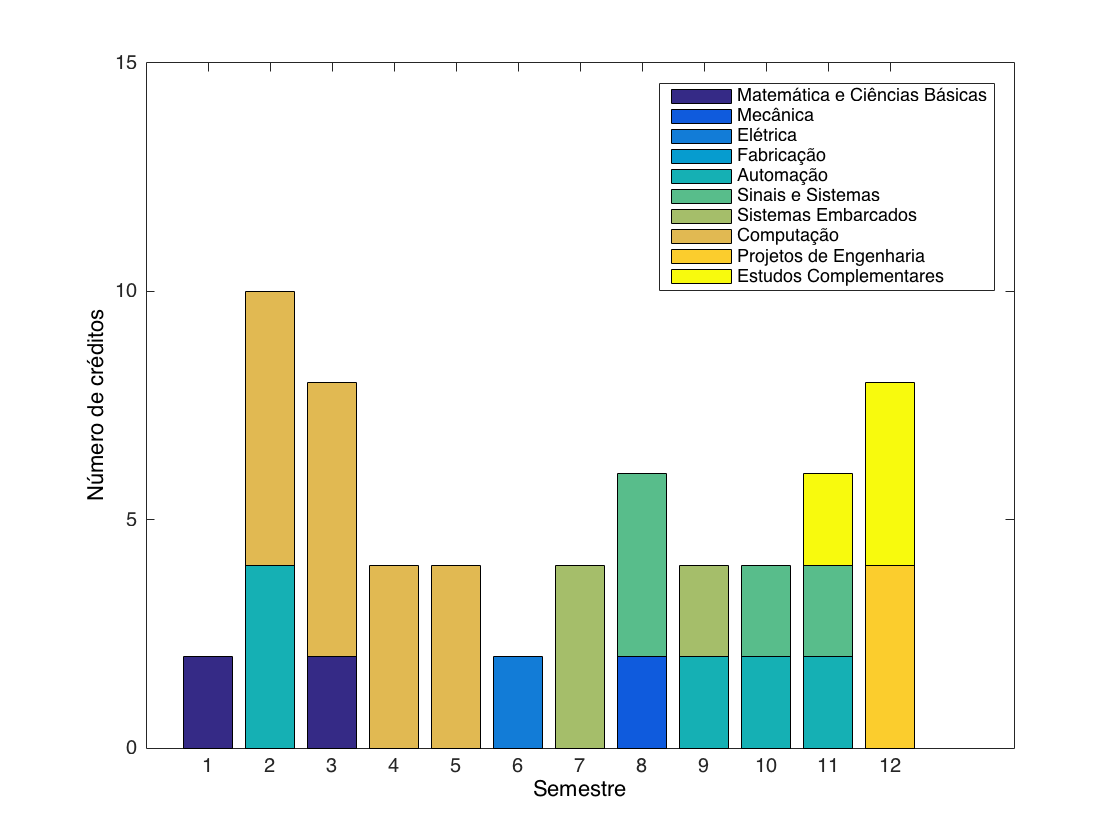
\includegraphics[scale=0.30]{pictures/graficoMaterias.png}\\


\paragraph{} O gráfico acima mostra a distribuição de matérias práticas ao longo do período de 12 semestres do curso. Pode-se observar uma concentração de matérias de computação no inicio do curso e uma de outras matérias no fim, porém o meio do curso (do quarto ao sétimo mestre) apresenta poucas matérias práticas.

%----------------------------------------------------------------------------------------
%	Outras Instituições
%----------------------------------------------------------------------------------------

\section{Outras Instituições}

\paragraph{} Tendo compilado as informações do curso de Engenharia de Controle e Automação da Unicamp, o próximo passo do estudo é analisar os cursos de outras instituições de ensino superior sob métricas semelhantes ou equivalentes. 

\paragraph{} Foram escolhidas três instituições de renome nacional e internacional, são elas:

\begin{itemize}
\item Universidade Federal de Itajubá (UNIFEI)
\item Massachusetts Institute of Technology (MIT)
\item University of Cambridge
\end{itemize}

\subsection{Universidade Federal de Itajubá}

\paragraph{} O curso de Engenharia de Controle e Automação da Universidade Federal de Itajubá foi fundado em 1998, mesmo ano que o curso da Unicamp, porém apresenta diferenças significativas em seu catalógo. De acordo com o seu projeto pedagógico, o curso tem como objetivo a: "formação de recursos humanos para o desenvolvimento científico e tecnológico de área de sistemas de controle e automação, assim como na aplicação de tecnologias que visam à melhoria de produtos e serviços em geral". 

\begin{figure}[H]
\centering

\includegraphics[scale=0.50]{pictures/fei.jpg}\\
\caption{Universidade Federal de Itajubá}

\end{figure}


\paragraph{} A estrutura do curso é explicitamente dividida entre disciplinas teóricas e práticas e pode-se ver uma preocupação em garantir uma carga horária prática em quase todos os semestres, sendo a exceção o ultimo semestre (usado para estágio e trabalho final de graduação). 

\paragraph{} Além das disciplinas abaixo, a universidade oferece disciplinas optativas em áreas como empreendedorismo, sistemas embarcados, análise de algoritmos, eletromagnetismo, engenharia de software, sistemas operacionais e outras áreas que não serão consideradas nessa análise, já que o foco deste trabalho se encontra na grade obrigatória.

\begin{table}[H]
\centering
\begin{tabular}{|c|l|c|}
\hline
Semestre             & Disciplina                                                 & Créditos \\ \hline
\multirow{5}{*}{1o}  
				   & Desenho Técnico Básico                                                  & 4        \\ \cline{2-3} 
                     & Metodologia Cientifica                                                     & 2        \\ \cline{2-3} 
                     & Introdução à Engenharia de Controle e Automação      & 2        \\ \cline{2-3} 
                     & Laboratório de Metodologia Cientifica						    & 1		\\ \cline{2-3} 
                     & Geometria Analítica e Algebra Linear                              & 4        \\ \cline{2-3} 
                     & Cálculo 1                                           								& 6       \\ \cline{2-3} 
                     & Química Geral																& 4       \\ \cline{2-3} 
                     & Química Experimental													& 1       \\ \hline
\multirow{5}{*}{2o}  
				   & Cálculo II                                                 & 4        \\ \cline{2-3} 
				   & Equações Diferenciais I                                                 & 4        \\ \cline{2-3} 
                     & Física Geral I                                          & 4        \\ \cline{2-3} 
                     & Física Experimental I                                      & 2        \\ \cline{2-3} 
                     & Desenho Técnico Auxiliado por Computador                   & 2        \\ \cline{2-3} 
                     & Circuitos Elétricos I                                     & 3        \\ \cline{2-3} 
                     & Laborátorio de Circuitos Elétricos I                                       & 1        \\ \cline{2-3} 
                     & Técnicas de Programação                   & 2         \\ \cline{2-3} 
                     & Laboratório Técnicas de Programação                   & 2        \\ \hline
\multirow{5}{*}{3o}  
					& Matemática Discreta                                       & 3        \\ \cline{2-3} 
				    & Laboratório de Matemática Discreta                                        & 2        \\ \cline{2-3} 
				    & Estruturas de Dados                                        & 3        \\ \cline{2-3} 
				    & Laboratório de Estruturas de Dados                                        & 2        \\ \cline{2-3} 
					& Circuitos Elétricos I                                     & 2        \\ \cline{2-3} 
                      & Laborátorio de Circuitos Elétricos II                                     & 1        \\ \cline{2-3} 
                      	& Introdução à Eletrônica Analógica                                     & 2        \\ \cline{2-3} 
                      & Laborátorio de Introdução à Eletrônica Analógica                                    & 1        \\ \cline{2-3} 
                      & Eletrônica Digital I                                     & 3        \\ \cline{2-3} 
                      & Laborátorio de Eletrônica Digital II                                  & 1        \\ \cline{2-3} 
					& Cálculo III                                                & 4        \\ \cline{2-3} 
                      & Equações Diferenciais II                                    & 4        \\ \hline
\end{tabular}
\caption{Catálogo 2017 UNIFEI -  Parte 1}
\label{catalago1}
\end{table}

\begin{table}[H]
\centering
\begin{tabular}{|c|l|c|}
\hline
Semestre             & Disciplina                                                 & Créditos \\ \hline

\multirow{5}{*}{4o}  
					& Modelagem de Sistemas Dinâmicos                                       & 3        \\ \cline{2-3} 
				    & Introdução à Análise de Sinais                                        			& 1        \\ \cline{2-3} 
				    & Teoria de Grafos                                        								& 2        \\ \cline{2-3} 
				    & Programação Orientada a Objetos                                          & 2        \\ \cline{2-3}
				    & Laboratórios de Programação Orientada a Objetos               & 2        \\ \cline{2-3}  
					& Circuitos Polifásicos                                   							& 3        \\ \cline{2-3} 
                      	& Eletrônica Analógica I                                     						& 3        \\ \cline{2-3} 
                      & Laborátorio de Eletrônica Analógica I                                   & 1        \\ \cline{2-3} 
                      & Eletrônica Digital II                                     & 2        \\ \cline{2-3} 
                      & Laborátorio de Eletrônica Digital II                                   & 1        \\ \cline{2-3} 
					& Física Geral III                                                & 4        \\ \cline{2-3} 
                      & Laboratório de Eletrônica Digital                                                 & 1        \\ \hline
\multirow{5}{*}{5o}  
					& Automação e Supervisórios I                                      			& 4        \\ \cline{2-3} 
				    & Controle Clássico                                        							& 4        \\ \cline{2-3} 
				    & Laboratório de Controle Clássico                                        	& 1        \\ \cline{2-3} 
				    & Instrumentação							                                             & 2        \\ \cline{2-3}
				    & Laboratórios de Instrumentação               							& 1        \\ \cline{2-3}  
					& Eletrônica de Potência e Acionamentos Controlados   			& 4        \\ \cline{2-3} 
                      & Laborátorio de Eletrônica de Potência e Acionamentos Controlados  & 1        \\ \cline{2-3} 
                      & Fenômenos de Transporte                                    & 4        \\ \cline{2-3} 
                      & Laborátorio de Fenômenos de Transporte                                   & 1        \\ \cline{2-3} 
					& Cálculo Numérico                                                & 4        \\ \hline
\multirow{6}{*}{6o} 
				   & Automação e Supervisórios II                         & 4        \\ \cline{2-3} 
                     & Controle Moderno e Avançado                           & 2        \\ \cline{2-3} 
                     & Laboratório de Controle Moderno e Avançado                           & 1        \\ \cline{2-3}
                     & Maquinas Elétricas                           & 4        \\ \cline{2-3} 
                     & Laboratório de Maquinas Elétricas                           & 1        \\ \cline{2-3}  
                     & Mecânica dos Sólidos                                 & 3        \\ \cline{2-3} 
                     & Processos de Transformação                                   & 4        \\ \cline{2-3} 
                     & Probabilidade e Estatística                                         & 4        \\ \hline					
\end{tabular}
\caption{Catálogo 2017 UNIFEI -  Parte 2}
\label{catalago1}
\end{table}

\begin{table}[H]
\centering
\begin{tabular}{|c|l|c|}
\hline
Semestre             & Disciplina                                                 & Créditos \\ \hline                                        
\multirow{6}{*}{7o}  
				   & Comunicação e Expressão                          		& 4        \\ \cline{2-3} 
                     & Gestão de Operações                           & 3        \\ \cline{2-3} 
                     & Sistemas e Eventos Discretos                                 & 4        \\ \cline{2-3} 
                     & Automação Pneumática e Hidráulica                          & 2        \\ \cline{2-3} 
                     & Laboratório de Automação Pneumática e Hidráulica                          & 2        \\ \cline{2-3} 
                     & Sistemas Integrados de Manufatura                          & 2        \\ \cline{2-3}  
                     & Controle Robusto e Multiváriavel                                & 4        \\ \cline{2-3} 
                     & Microcontroladores e Microprocessadores                        & 2        \\ \cline{2-3} 
                     & Laboratório de Microcontroladores e Microprocessadores                            & 2        \\ \hline

\multirow{6}{*}{8o}  
				   & Ciências do Ambiente                          		& 4        \\ \cline{2-3} 
                     & Introdução a Robótica                          & 3        \\ \cline{2-3} 
                     & Banco de Dados para Automação                                & 3        \\ \cline{2-3} 
                     & Identificação de Sistemas e Técnicas Avanças de Controle                          & 4        \\ \cline{2-3} 
                     & Economia                          & 3        \\ \cline{2-3} 
                     & Materiais Elétricos e Eletrônicos                         & 2        \\ \cline{2-3}  
                     & Redes Industriais                                & 4        \\ \cline{2-3} 
                     & Laboratório de Redes Industriais                            & 1.5        \\ \hline  
\multirow{6}{*}{9o}  
				   & Projetos de Sistemas de Automação                          		& 2        \\ \cline{2-3} 
                     & Planejamento e Gestão da Qualidade                          & 3        \\ \cline{2-3} 
                     & Engenharia Econômica                               & 3        \\ \cline{2-3} 
                     & Ciências Humanas e Sociais                          & 3        \\ \hline
\multirow{6}{*}{10o}  
				   & Projetos de Sistemas de Automação                          		& 2        \\ \cline{2-3} 
                     & Ciências Humanas e Sociais                          & 3        \\ \hline

\end{tabular}
\caption{Catálogo 2017 UNIFEI -  Parte 3}
\label{catalago1}
\end{table}

O curso oferece $205.5$ créditos obrigatórios, aonde $49.5$ são créditos que oferecem experiência prática aos alunos. O que corresponde à $24.10\%$ do curso, um percentual semelhante ao curso da Unicamp, porém avaliando a distribuição desses créditos nas grupos definidos anteriormente:

\begin{table}[H]
\centering
\resizebox{\textwidth}{!}{
\begin{tabular}{|p{3cm}|p{7cm}|c|p{2cm}|p{2.5cm}|p{3cm}|}
\hline
Grupo & Disciplinas & Créditos & Créditos Práticos & Porcentagem do Curso & Porcentagem dentro da parte prática \\ \hline

Matemática e Ciências Básicas & {Calculo I, Geometria Analítica e Álgebra Linear, Cálculo II, Equações Diferenciais I, Matemática Discreta, Laboratório de Matemática Discreta, Cálculo III, Equações Diferenciais II, Cálculo Numérico, Probabilidade e Estatística, Química Geral, Química Experimental, Física Geral I, Física Experimental I, Física Geral III, Física Experimental III} & 53 & 4  & 25.8\%  & 8.1\% \\ \hline

Mecânica & {Fenômenos de Transporte, Laborátorio de Fenômenos de Transporte, Mecânica dos Sólidos} & 8 & 1 & 3.9\% & 2\% \\ \hline

Elétrica & {Circuitos Elétricos I, Laboratório de Circuitos Elétricos I, Circuitos Elétricos II, Laboratório de Circuitos Elétricos II, Introdução à Eletrônica Analógica, Laboratório de Introdução à Eletrônica Analógica, Circuitos Polifásicos, Eletrônica Analógica I, Laboratório de Eletrônica Analógica I, Materiais Elétricos e Eletrônicos} & 19 & 4 & 9.3\% & 8.1\% \\ \hline

Fabricação & {Desenho Técnico Básico, Desenho Técnico Auxiliado por Computador, Processos de Transformação, Sistemas a Eventos Discretos, Sistemas Integrados de Manufatura} & 16 & 6 & 7.8\% & 12.1\% \\ \hline

Automação & {Modelagem de Sistemas Dinâmicos, Automação e Supervisórios I, Instrumentação, Laboratório de Instrumentação, Eletrônica de Potência e Acionamentos Controlados, Laboratório de Eletrônica de Potência e Acionamentos Controlados, Automação e Supervisórios II, Máquinas Elétricas, Laboratório de Máquinas Elétricas, Automação Pneumática e Hidráulica, Laboratório de Automação Pneumática e Hidráulica, Introdução a Robótica, Banco de Dados para Automação, Redes Industriais, Laboratório de Redes Industriais}
& 39.5 & 17.5 & 19.2\% & 35.4\% \\ \hline


\end{tabular}
}
\caption{Divisão das disciplinas em grandes grupos - Parte 1}
\label{div1}
\end{table}

\begin{table}[H]
\centering
\resizebox{\textwidth}{!}{
\begin{tabular}{|p{3cm}|p{7cm}|c|p{2cm}|p{2.5cm}|p{3cm}|}
\hline
Grupo & Disciplinas & Créditos & Créditos Práticos & Porcentagem do Curso & Porcentagem dentro da parte prática \\ \hline

Sinais e Sistemas & {Introdução à Análise de Sinais, Controle Clássico, Laboratório de Controle Clássico, Controle Moderno Avançado, Laboratório de Controle Moderno Avançado, Controle Robusto e Multivariável, Identificação de Sistemas e Técnicas Avançadas de Controle} & 17 & 4 & 8.3\% & 8.1\% \\ \hline

Sistemas Embarcados & {Eletrônica Digital I, Laboratório de Eletrônica Digital I, Eletrônica Digital II, Laboratório de Eletrônica Digital II, Microcontroladores e Microprocessadores, Laboratório de Microcontroladores e Microprocessadores} & 11 & 4 & 5.4\% & 8.8\% \\ \hline

Computação & {Técnicas de Programação, Laboratório de Técnicas de Programação, Estrutura de Dados, Laboratório de Estrutura de Dados, Teoria de Grafos,Programação Orientada a Objetos, Laboratório de Programação Orientada a Objetos } & 15 & 6 & 7.3\% & 29.2\%  \\ \hline

Projetos de Engenharia & {Introdução à Engenharia de Controle e Automação I, Projeto de Sistemas de Automação, Trabalho Final de Graduação} & 4 & 2 & 1.9\% & 4.1\%\\ \hline

Estudos Complementares & {Metodologia Científica, Laboratório de Metodologia Científica, Comunicação e Expressão, Gestão de Operações, , Ciências do Ambiente, Economia, Planejamento e Gestão da Qualidade, Engenharia Econômica, Ciências Humanas e Sociais} & 23 & 1 & 11.2\% & 2.1\% \\ \hline

\end{tabular}
}
\caption{Divisão das disciplinas em grandes grupos - Parte 2}
\label{div1}
\end{table}

\paragraph{} A tabela acima mostra que o curso oferecido pela UNIFEI possui uma enfâse maior no grupo de Automação comparado com a Unicamp, porém todos os outros grupos apresentam um número parecido de créditos práticos, mostrando um maior equilibrio neste ponto. Agora, distribuindo estas disciplinas em seus respectivos semestres:

\begin{figure}[H]
\centering
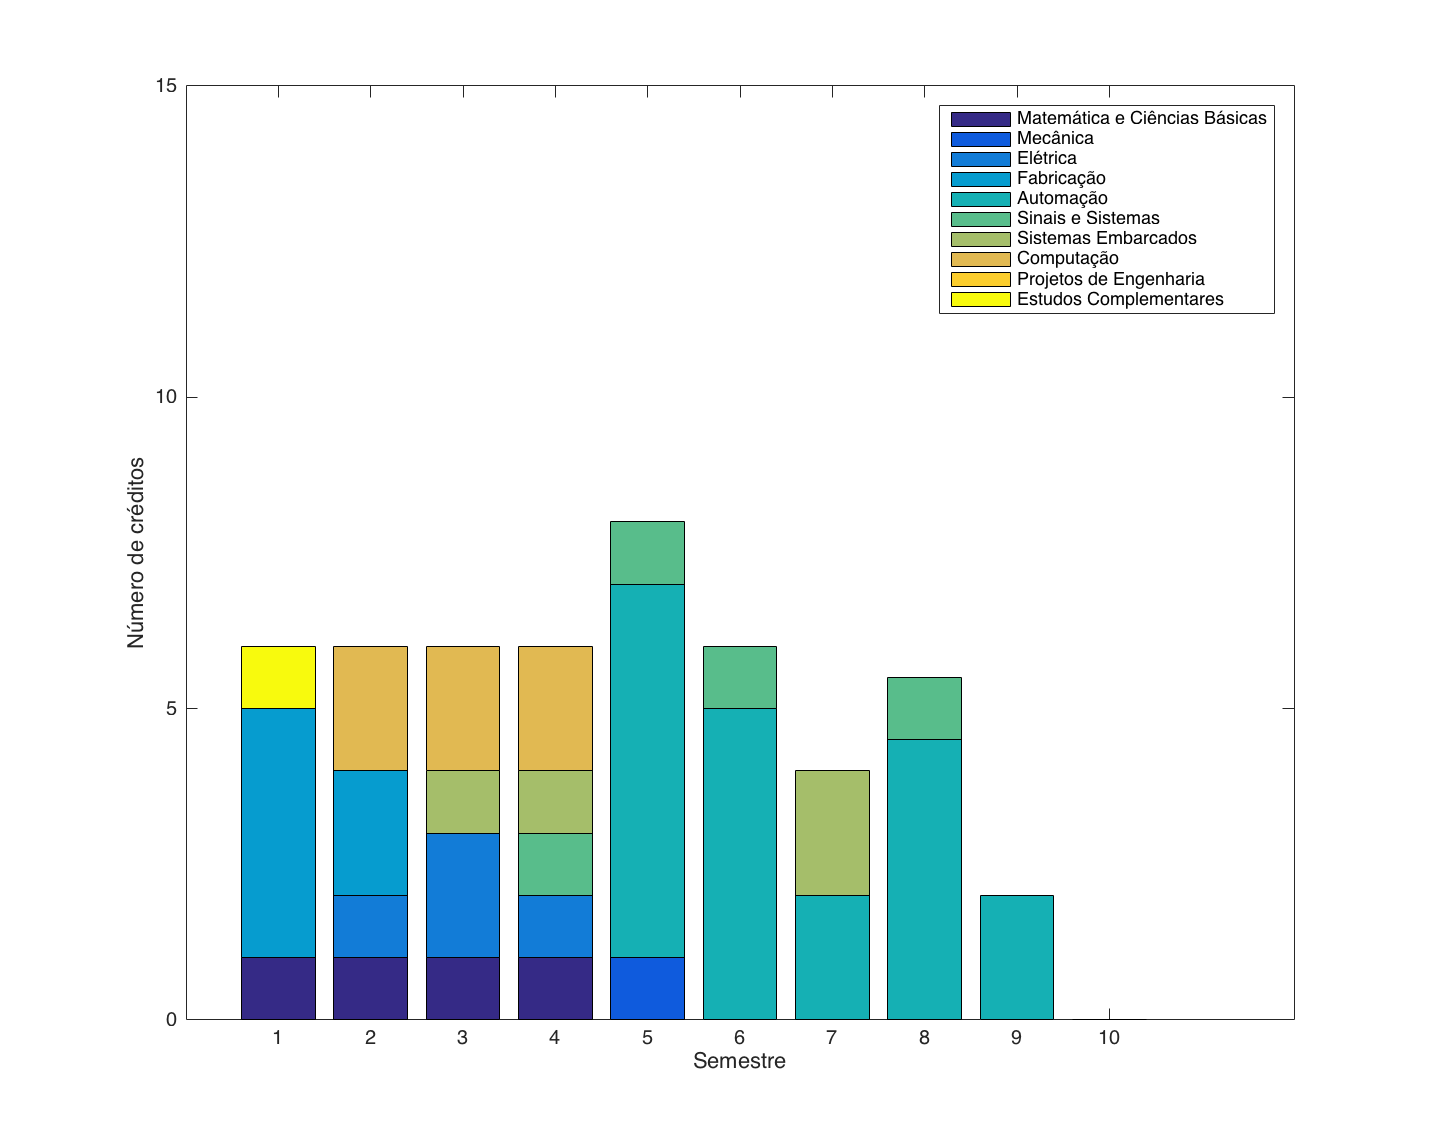
\includegraphics[scale=0.3]{pictures/graficoFei.png}\\
\caption{Divisão dos créditos práticos nos períodos do curso}

\end{figure}

\paragraph{} Nota-se uma diferença da distribuição dos créditos práticos na Unicamp. Apesar de haver uma predominancia do grupo de Automação, os créditos estão igualmente distribuidos por todos os semestres, oferecendo contato com diferentes competências práticas durante quase toda a graduação (a exceção sendo o último ano).

\paragraph{} A abordagem da UNIFEI de separar os créditos práticos por toda a graduação permite que os alunos nunca fiquem sobrecarregados de matérias práticas e tenham contato com elas durante o curso inteiro.

%----------------------------------------------------------------------------------------
%	MIT
%----------------------------------------------------------------------------------------


%----------------------------------------------------------------------------------------
%	Cambridge
%----------------------------------------------------------------------------------------

\subsection{Cambridge University}

\paragraph{} O curso de graduação em Engenharia pela Cambridge University é dividido em quatro partes.

\paragraph{} Durante a primeira parte, com duração de dois anos, os alunos tem aulas téoricas nos campos de : Mecânica, Estruturas, Materiais, Mecânica dos Fluidos, Termodinamica, Elétrica, Eletrônica, Computação, Controle e Matematica. Durante este período os alunos devem fazer duas horas de experimentos em laboratório por semana além de exercícios de desenho técnico, computação, e projetos na área de design de estruturas, integração elétrica em um laboratório de robótica, projeto de integração sobre estruturas em terremotos e mini-projetos de caracterização de materiais.

\paragraph{} Na segunda parte do grupo, o aluno pode escolher uma área de especialização ou se manter em uma área mais abrangente. As especializações são: Aeroespacial e Aerotérmica, Mecanica, Bioengenharia, Civil, Ambiental, Energia, Estruturas, Elétrica e Eletrônica, Elétrica e Ciência da Informação, Computação e Informação, Instrumentação e Controle.
%----------------------------------------------------------------------------------------
% MIT
%----------------------------------------------------------------------------------------

\subsection{MIT}

%----------------------------------------------------------------------------------------
%	Próximos Passos
%----------------------------------------------------------------------------------------

\section{Próximos passos}

\paragraph{} Tendo compilado as informações do curso de Engenharia de Controle e Automação da Unicamp, o próximo passo do estudo é analisar os cursos de outras instituições de ensino superior sob as mesmas métricas. Planeja-se entrar em contato com universidades de renome internacional, analisar o curriculo proposto e também entender as propostas para matérias de desenvolvimento de projeto.

\paragraph{} Com as informações de outras instituições de ensinos, será possível comparar ambas as realidades (Unicamp e outras universidades) e entender quais as mudanças necessárias para que o problema de falta de contato técnico seja sanado, também procura-se alinhar o curso da Unicamp aos cursos de outras instituições de prestigio internacional, porém sem perder de vista a realidade brasileira.


\bibliographystyle{apa}
 \bibliography{../bibliografia/bibliografia}

\end{document}